\documentclass{article}
\usepackage[T1]{fontenc}
\usepackage{lmodern}
\usepackage{graphicx}
\usepackage{amsmath,amssymb}
\usepackage[a4paper,margin=2cm]{geometry}
\usepackage[absolute,overlay]{textpos}
\setlength{\TPHorizModule}{1mm}
\setlength{\TPVertModule}{1mm}
\usepackage[indonesian]{babel}
\usepackage{hyperref}
\setlength{\emergencystretch}{2em}
% unit: Halaman 6

\begin{document}

% === Halaman 6 (llm) ===

\vspace{225.72mm}

\begin{itemize}
  \item Konversi teks ke biner: \url{https://www.rapidtables.com/convert/number/string-to-binary.html}
\end{itemize}
\vspace{10mm}

% deskripsi: Screenshot halaman web RapidTables yang menunjukkan alat konversi teks ke biner dengan input 'Halo' dan output binernya.
% bbox normalisasi: [0.0780, 0.1500, 0.5300, 0.9100]
\begin{textblock*}{94.92mm}(16.38mm,44.55mm)
\noindent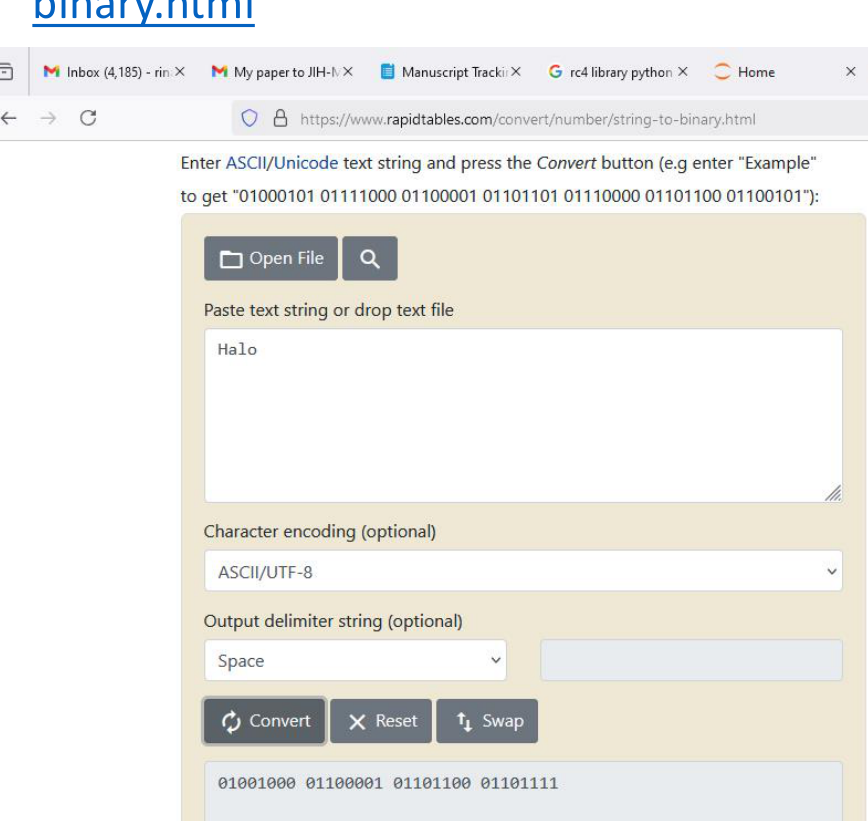
\includegraphics[width=94.92mm,height=225.72mm]{../../images/llm/page_006_img_01.png}%
\end{textblock*}

\end{document}
